\documentclass[a4, english, twoside]{article}
% a4 is the paper size
% english is for the language used in standard texts (figures, tables etc)
% twoside for doublesided pages. Remove if that is not wanted.

%%%%%%%%%%%%%%%%%%%%%%%%%
% Load Preample         %
%%%%%%%%%%%%%%%%%%%%%%%%%

%Import from the same folder
%%%%%%%%%%%%%%%%%%%%%%%%%%%%%%%%%%%%
% Settings for document (english) %
%%%%%%%%%%%%%%%%%%%%%%%%%%%%%%%%%%%

% Input common definition
%%%%%%%%%%%%%%%%%%%%%%%%%%%%%%%%
%    Papersize and encoding    %
%%%%%%%%%%%%%%%%%%%%%%%%%%%%%%%%

% Size of margins can be changed here in the outcommented version!
%\usepackage[a4paper, total={6in, 8in}]{geometry}	%total={width, height}
\usepackage[a4paper]{geometry}

% Basics: font, codec etc.
\usepackage[utf8]{inputenc}						% encoding: utf-8 (nordic letters)
\usepackage[T1]{fontenc}						% use 8-bit encoded fonts
\renewcommand{\sfdefault}{phv}					% changes the default font

%\usepackage[parfill]{parskip}      %Instead of indenting on a newline adds whitespace



%%%%%%%%%%%%%%%%%%%%%%%%%%%%%%%%
%      Tables and figures      %
%%%%%%%%%%%%%%%%%%%%%%%%%%%%%%%%

\usepackage{tabularx,booktabs,authblk}		    % various basic stuff for tables and more

% Figures and captions
\usepackage{caption}							% create captions for figures
\usepackage{subfig}								% create subfigures of a figure
%\usepackage{subcaption}					% create captions for subfigures
                                  %     currently off, due to conflicts

\usepackage{wrapfig}							% letting figures be in text

\usepackage{rotating}             % let any environment be rotated (figures sideways)
                                  %     \begin{sideways} or \begin{turn}{30}



%%%%%%%%%%%%%%%%%%%%%%%%%%%%%%%%%%%%
%           Variables              %
%%%%%%%%%%%%%%%%%%%%%%%%%%%%%%%%%%%%
\usepackage{pgfkeys}			%Initialize the variable key-value parirs

\newcommand{\setvalue}[1]{\pgfkeys{/variables/#1}}
\newcommand{\getvalue}[1]{\pgfkeysvalueof{/variables/#1}}
\newcommand{\declare}[1]{%
 \pgfkeys{
  /variables/#1.is family,
  /variables/#1.unknown/.style = {\pgfkeyscurrentpath/\pgfkeyscurrentname/.initial = ##1}
 }%
}

\declare{}



%%%%%%%%%%%%%%%%%%%%%%%%%%%%%%%%
%      LaTeX Programming       %
%%%%%%%%%%%%%%%%%%%%%%%%%%%%%%%%

\usepackage{xparse}								% Scanning arguments
\usepackage{xifthen}							% Conditionals
\usepackage{xstring}                            % String functions
\usepackage{calc}								% Calculations



%%%%%%%%%%%%%%%%%%%%%%%%%%%%%%%%
%          Hypermedia          %
%%%%%%%%%%%%%%%%%%%%%%%%%%%%%%%%

\usepackage{url, hyperref}							% \url{link} and \href{link}{replacing text}

%Macros taken from the preamble of the MatFysTutor LaTeX Guide.
\newcommand*{\http}[1]{\href{http://#1}{#1}}		% macro for http links: \http{www.matfystutor.dk}
\newcommand*{\mailto}[1]{\href{mailto:#1}{#1}}		% macro for mails: \mailto{email@email.com}

%%%%%%%%%%%%%%%%%%%%%%%%%%%%%%%%
%         Stylization          %
%%%%%%%%%%%%%%%%%%%%%%%%%%%%%%%%

% Headers og footers
\usepackage{lastpage}                           % \lastpage command for numbers of pages
\usepackage{fancyhdr}                           % create cool headers and footers
\pagestyle{fancy}                               % who doesn't want their page to be fancy?

% Use of columns
\usepackage{multicol}

% Quotations
% "danish" or "british"
\usepackage[danish=guillemets]{csquotes}    	% two styles: "quotes" or >>guillemets<<
%\MakeAutoQuote{»}{«}                       	% decomment for easy macro
%\MakeAutoQuote*{›}{‹}                      	% decomment for even easier macros

% Like a paragraph, but adds also a linebreak after. (Also is not recorded on labelling)
\newcommand{\lbparagraph}[1]{\vspace{0.3em} \noindent \textbf{#1}\\ \noindent}

% Underlining and strikethrough text
\usepackage[normalem]{ulem}

%%%%%%%%%%%%%%%%%%%%%%%%%%%%%%%%
%             Math             %
%%%%%%%%%%%%%%%%%%%%%%%%%%%%%%%%
%\newcommand{\hmmax}{0}								% minimizes the amount of bold families
%\newcommand{\bmmax}{1}								% this allows for more math families

% various basic stuff
\usepackage{mathtools, amsmath}
\allowdisplaybreaks                                 % allow pagebreaks in align* ?

% other math goodies
\usepackage{cancel}

% Various symbol packages
\usepackage{amssymb}
\usepackage[utopia]{mathdesign}					    % full overwrite of the font system
\usepackage{stmaryrd}								% even more symbols

\DeclareMathAlphabet{\mathpzc}{OT1}{pzc}{m}{it}     % \mathpzc a less pompous curly typeset

% Math shortcuts
\renewcommand{\d}{\, \mathrm{d}}                    % \d = differential d with a bit of spacing
\newcommand{\e}{\mathrm{e}}                         % \e = eulers number
\newcommand{\R}{\mathbb{R}}                         % \R = Real numbers
\newcommand{\N}{\mathbb{N}}                         % \N = Natural numbers
\newcommand{\C}{\mathbb{C}}                         % \C = Complex numbers
\newcommand{\Q}{\mathbb{Q}}                         % \Q = Rational numbers
\newcommand{\F}{\mathbb{F}}							% \F = Field
\newcommand{\K}{\mathbb{K}}							% \K = Field \R and \C
\newcommand{\V}{\mathpzc{V}}						% \V
\newcommand{\W}{\mathpzc{W}}						% \W
\renewcommand{\S}{\mathbb{S}}						% \S = Set of permutations

\newcommand{\Det}[1]{\text{Det}\left( #1 \right)}   % \Det{arg}             Det(arg)
\newcommand{\Span}[1]{\text{Span}\left( #1 \right)} % \Span{arg}			Span(arg)
\newcommand{\sgn}[1]{\text{sgn} \left( #1 \right)}  % \sgn{arg}				sng(arg)
\newcommand{\adj}[1]{\text{adj} \left( #1 \right)}  % \adj{arg}             adj(arg)

\newcommand{\abs}[1]{\left\lvert #1 \right\rvert}			% \abs{arg}		absolute/modulo of value
\newcommand{\norm}[1]{\left\lVert #1 \right\rVert}			% \norm{arg}	norm of a value
\newcommand{\ceil}[1]{\left\lceil #1 \right\rceil}			% \ceil{arg}	ceiling of a value
\newcommand{\floor}[1]{\left\lfloor #1 \right\rfloor}		% \floor{arg}	floor of a value
\newcommand{\inprod}[2]{\left\langle #1 , #2 \right\rangle}	% \inprod{arg}	inner product

\newcounter{i}

\DeclareDocumentCommand \seq { g g g g } {			% \seq{x}{i}{j}{s}
	\setcounter{i}{0}								% x_i, x_i+s, ... x_j
	\IfValueT {#2} { \addtocounter{i}{#2} }
	\IfValueTF {#1}
		{#1}
		{x}
	_{ \arabic{i} },
	\IfValueTF {#4} 
		{\addtocounter{i}{#4}}
		{\addtocounter{i}{1}}
	\IfValueTF {#1} 
		{#1}
		{x} 
	_{ \arabic{i} },
	\dots
	\IfValueTF {#3}
		{ , #1_{#3} }
		{}
}

\DeclareDocumentCommand \ero { g g } {				% \ero {x, y}
	\begin{array}{c}								%	x
		\IfValueTF{#1}								%	~
			{_{#1}}									%	y
			{\phantom{\sim}}
	\\
		\sim
	\\
		\IfValueTF{#2}
			{^{#2}}
			{\phantom{\sim}}
	\end{array}
}

\DeclareDocumentCommand \coorvec { m g }{			% \coorvec{v}{V}	Coordinate vector
	\left[
		#1
	\right]
	{_{
		\IfValueTF{#2}
			{#2}
			{\epsilon}
	}}
}

\DeclareDocumentCommand \matrep { g g g } {			% \matrep{W}{L}{V}	Matrixrepresentation
	{_{												% W[L]V
		\IfValueTF {#1}									%No arguments for W or V results in standardbasis
			{#1}										%No arguments for L results in coordinatetransformation
			{\epsilon}
	}}
	\left[
		\IfValueTF {#2}
			{#2}
			{\square}
	\right] {_{
		\IfValueTF {#3}
			{#3}
			{\epsilon}
	}}
}

\DeclareDocumentCommand \set { m g }{ 				% \sets{X}{C}
	 \left\lbrace									% {X | C}
	 	#1 \IfValueT {#2} { \ | \  #2 }
	 \right\rbrace
}

\makeatletter										% adds vertical lines to matrices
\renewcommand*\env@matrix[1][*\c@MaxMatrixCols c]{
  \hskip -\arraycolsep
  \let\@ifnextchar\new@ifnextchar
  \array{#1}}
\makeatother

%%%%%%%%%%%%%%%%%%%%%%%%%%%%%%%%
%      Logic and proofs        %
%%%%%%%%%%%%%%%%%%%%%%%%%%%%%%%%

% Proofs
\usepackage{amsthm}								% Theorem package
\theoremstyle{definition}						% plain, definition, remark
%\swapnumbers									% If you want to have the number first

% Logic packages
\usepackage{lplfitch}						% fitch style proofs

%\usepackage{logicproof}					% alternative package, resembling the dBerLog book
%\setlength\subproofhorizspace{2em}			% Indent for subproofs. Changed for fresh variables



%%%%%%%%%%%%%%%%%%%%%%%%%%%%%%%%
%      Color and presets       %
%%%%%%%%%%%%%%%%%%%%%%%%%%%%%%%%

%\usepackage{xcolor}							% basic xcolor package
\usepackage[table,xcdraw]{xcolor}				% xcolor package with support for tables
\usepackage{colortbl}                           % color presets working together with xcolor

\definecolor{lstComment}{rgb}{0.45,0.45,0.45}	% code: comments (Grey)
\definecolor{lstKey}{rgb}{0.13,0.21,1}			% code: primary keywords (Blue)
\definecolor{lstKey2}{rgb}{1,0.666667,0.13726}  % code: secondary keywords (Day[9] Orange)
\definecolor{lstString}{rgb}{0.1,0.65,0.1}		% code: strings (Green)
\definecolor{lstBase}{rgb}{0.0,0.0,0.0}			% code: base (Black)



%%%%%%%%%%%%%%%%%%%%%%%%%%%%%%%%
%            Tikz              %
%%%%%%%%%%%%%%%%%%%%%%%%%%%%%%%%

\usepackage{tikz}								% import basepackage
\usetikzlibrary{calc}							% Coordinate calcuations
\usetikzlibrary{positioning}                    % Relative positioning
\usetikzlibrary{shapes}                         % Defining nodeshapes and more (isa for E/R)

% Simple tree macro with compability to tikz
\usepackage{tikz-qtree}							% import simple tree macro
\usetikzlibrary{arrows}                         % arrows for trees

% Tikz settings for red-black trees
\tikzset{
  treenode/.style = {align=center, inner sep=0pt, text centered,
    font=\sffamily},
  arn_b/.style = {treenode, circle, white, font=\sffamily\bfseries, draw=black,
    fill=black, text width=1.5em},              % black node
  arn_r/.style = {treenode, circle, white, font=\sffamily\bfseries, draw=red,
    fill=red, text width=1.5em},              % red node
  arn_x/.style = {treenode, rectangle, draw=black, fill=black,
    minimum width=0.5em, minimum height=0.5em}  % nil node
}

% Tikz Automota for Turing Machines
\usetikzlibrary{automata}

% Tikz E/R diagram
\usetikzlibrary{er}

% Graphics and plots
\usepackage{graphicx}							% import basepackage for graphs
\usepackage{pgfplots}							% import pgfplots
\usepgfplotslibrary{fillbetween}				% add fillBetween command
\pgfplotsset{compat=1.10}						% choose version of pgfplots

% Macro for circle with symbol inside.
\newcommand*\circled[1]{ \tikz[baseline=(C.base)]\node[draw,circle,inner sep=0.5pt](C) {#1};\!}



%%%%%%%%%%%%%%%%%%%%%%%%%%%%%%%%
%            Code              %
%%%%%%%%%%%%%%%%%%%%%%%%%%%%%%%%
\newcommand{\code}[1]{{\sf #1}}					% \code{X} writes X in a code-appropriate font




%%%%%%%%%%%%%%%%%%%%%%%%%%%%%%%%
%         lstlisting           %
%%%%%%%%%%%%%%%%%%%%%%%%%%%%%%%%

% Import lstlistings - beautiful sourcecode!
\usepackage{listings}


% Custom language definitions
% Definition of Pseudocode
\lstdefinelanguage{pseudocode}{
  keywords=[1]{
  	     break, break, by, do, downto, else, error, for, if, repeat, return, to, until, while, while
  	},								    		% list of keywords, first and last are not used for some stupid reason
  keywords=[2]{
        and, and, or, NIL, NIL
  }
  sensitive=false,								% keywords are not case-sensitive
  morecomment=[l]{//},							% l is for line comment
  morecomment=[s]{/*}{*/},						% s is for start and end delimiter
  morestring=[b]"								% strings are enclosed in double quotes
}


% Settings for lstlistings
\lstset{language=pseudocode,					% choose language
  columns=flexible,								% let the box align to the width of the page
    literate={æ}{{\ae}}1{ø}{{\o}}1{å}{{\aa}}1	% allow æ, ø and å in code
           {Æ}{{\AE}}1{Ø}{{\O}}1{Å}{{\AA}}1,	% 	(this change was taken from the preamble of the MatFysTutor LaTeX Guide)
  breaklines=true,								% automatically break lines
  breakatwhitespace=true,						% automatically break should there only be white space.
  numbers=left,									% numbering: none, left, right
  numbersep=5pt,								% distance between linenumbers and code
  numberstyle=\color{lstComment},				% change style of numbering - currently grey.
  stepnumber=1,									% step between to line-numbers. 1 = each line is numbered
  showspaces=false,								% show spaces everywhere - adding particular underscores
  showstringspaces=false,						% underline spaces within strings only.
  showtabs=false,								% show tabs within strings adding particular underscores.
  escapeinside={*@}{@*},                		% if you want to add LaTeX within your code
  basicstyle=\ttfamily \color{lstBase},			% set basic color
  commentstyle=\color{lstComment},				% set color of comments
  keywordstyle=[1]\color{lstKey},				% set color of primary keywords
  keywordstyle=[2]\color{lstKey2},				% set color of secondary keywords
  stringstyle=\color{lstString},				% set color of strings
}

% lstlisting - Put it beautifully in the middle
\lstset{xleftmargin= .1\textwidth ,     							% leftmargin being 10% of the current width
  xrightmargin= .1\textwidth,           							% right margin also 10%
  frame=bottomline                      							% Draw a line on the bottom of the surrounding box
}

% lstlisting header
\DeclareCaptionFont{white}{\color{white}}                                       % fontstyle of caption
\DeclareCaptionFormat{listing}{\colorbox{gray}{\parbox{\linewidth}{#1#2#3}}}    % create nice grey boxes for captions
\captionsetup[lstlisting]{format=listing,labelfont=white,textfont=white}        % apply settings to listing


%%%%%%%%%%%%%%%%%%%%%%%%%%%%%%%%%%%%
%      Title and information       %
%%%%%%%%%%%%%%%%%%%%%%%%%%%%%%%%%%%%
\setvalue{title = }
\setvalue{subtitle = }

\DeclareDocumentCommand \settitle { m g }{ 				% \setTitle{title}{subtitle}
	 \setvalue{title = #1}
	 \IfValueTF {#2} { \setvalue{subtitle = #2} \title{\huge \getvalue{title} \\ \large \getvalue{subtitle}}}
	 				 { \title{\huge \getvalue{title}} }
}

\DeclareDocumentCommand \addauth { m g g }{ 			% \addAuth{name}{email}{id}
     \IfValueT {#3} {		%Set the id text as desired on the top left
	 	\setvalue{id = #3}
	 }
     \pgfkeysifdefined{/variables/name}{
         \setvalue{id = \, et al}
     }{
         \setvalue{name = #1}
     }	 
	 \author{#1}
	 \IfValueT {#2} {
	    \pgfkeysifdefined{/variables/email}{
	        % Do Nothing
	    }{
	 	    \setvalue{email = #2}
	 	}
	 	\affil{\protect\href{mailto:#2}{#2}}
	 }
}

\settitle{Keep Calm and \textbackslash settitle}

\date{\today}

%Headers:
%  Unused pieces of code
%     Name of writers   \protect\href{\getvalue{email}}{\getvalue{name}\getvalue{id}}
%     "of X pages"      \getvalue{of} \pageref{LastPage}

%Odd pages (Main for onesided)

\fancyhead[LO]{\thepage}
\fancyhead[RO]{\getvalue{title}}

%Even pages
\fancyhead[LE]{\nouppercase{\leftmark}}
\fancyhead[RE]{\thepage}

%Nothing below
\fancyfoot[LCR]{}



%%%%%%%%%%%%%%%%%%%%%%%%%%%%%%%%
%   Encoding and hyphenation   %
%%%%%%%%%%%%%%%%%%%%%%%%%%%%%%%%
% Basics: font, codec etc.
\usepackage[english]{babel}                       % babel is for hyphenation and other goodies



%%%%%%%%%%%%%%%%%%%%%%%%%%%%%%%%
%         lstlisting           %
%%%%%%%%%%%%%%%%%%%%%%%%%%%%%%%%
\renewcommand{\lstlistingname}{Code}              % for one block of code alone
\renewcommand{\lstlistlistingname}{List of code}  % for more pieces of code in one



%%%%%%%%%%%%%%%%%%%%%%%%%%%%%%%%
%      Logic and proofs        %
%%%%%%%%%%%%%%%%%%%%%%%%%%%%%%%%
% Theorem environments
\newtheorem{theorem}{Theorem}[section]
\newtheorem{lemma}[theorem]{Lemma}
\newtheorem{proposition}[theorem]{Proposition}
\newtheorem{corollary}[theorem]{Corollary}
\newtheorem{definition}[theorem]{Definition}
\newtheorem{conjecture}[theorem]{Conjecture}
\renewcommand*{\proofname}{Proof}



%%%%%%%%%%%%%%%%%%%%%%%%%%%%%%%%
%      Example environment     %
%%%%%%%%%%%%%%%%%%%%%%%%%%%%%%%%
\newtheorem{example}[theorem]{Example}

%Import from absolute path
%\usepackage{import}
%\import{C:/GitHub/LaTeX_Preamble_and_Examples/preamble/}{preamble_dk.tex}

%Import from a relative path
\usepackage{import}
\subimport{../preamble/}{preamble_en.tex}

%%%%%%%%%%%%%%%%%%%%%%%%%
% Document starts here! %
%%%%%%%%%%%%%%%%%%%%%%%%%

\begin{document}

% Define title and more on frontpage
    \settitle{Examples Document}{Reverse engineerable \LaTeX}
    \addauth{Steffan Sølvsten}{201505832@post.au.dk}{\, au534068}
\maketitle

\begin{abstract}
\noindent The following document is meant to show the use of the various packages used in the preamble. They are all created with the intent to be reverse engineerable.
\end{abstract}

%En indholdsfortegnelse kan nemt laves med \tableofcontents funktionen
\tableofcontents

\newpage
\section{Math} \label{sec:math}
Most basically you use \emph{equation} to write a mathematical equation on a single new and centered line or you can write math in the text by writing \$ x\_0 \$ = $x_0$. If you want to write math over more lines, it is better to use the \emph{align} or even better the \emph{alignat} commands. In the following example with \emph{alignat}, we get the ability to align on more things, such that both the arrows on the left and the equals sign are aligned nicely. Here is a reference to line \ref{alignatL2}.

\begin{alignat}{2}
    && \cos x &= \cos x * \cos y \label{alignatL1}
    \\ \ArrowBetweenLines
    && 0 &= \cos x * \cos y - \cos x \label{alignatL2}
\intertext{
    Here is a line in the middle of the \emph{alignat}. So you can put in text between lines, but still keep the alignment across. This also gets linenumber except due to the \emph{nonumber}
}    \nonumber
    \\ \ArrowBetweenLines
    && 0 &= \cos x \cdot (\cos y - 1) \label{alignatL3}
\end{alignat}

\subsection{Matrices and vectors}
With \emph{pmatrix} matrices can also be made, such as in the following. For the row operations I have made the \emph{ero} macro to make life easier.
\begin{equation*}
    \begin{pmatrix}[cc|c]
        2 & 1 & 1
    \\
        1 & 1 & 0
    \end{pmatrix}
    \ero{R_1 - R_2}{2R2}
    \begin{pmatrix}[cc|c]
        1 & 0 & 1
    \\
        2 & 2 & 0
    \end{pmatrix}
\end{equation*}

\subsection{Alphabets}
In mathmode you can also use different styles called alphabets. Bold $\mathbf{b}$ and functions can be written with $\mathit{function}$. Furthermore the real numbers $\mathbb{R}$ has a shortcut $\backslash$ R and the same goes for $\C$, $\Q$, $\F$ and more. Finally with \emph{mathcal} you can get caligraphic writing, but if it is too pompous you can use \emph{mathpzc} for something looking like $\mathpzc{F, V, W}$.

Do note though, that using many different mathalphabets will at some point result in a compile error, since \LaTeX\ only can handle 16 mathalphabets and many are apparently already used up by many different packages. I have yet not tried to clean up, but hopefully you should not need that many different ways of writing the same letters.

\subsection{Other stuff}
Things like sequences and sets we use all the time too, which is why I've made macros. For a sequence you can write $\seq{a}{1}{n}{2}$ and for sets $ \set{x \in \Sigma^*}{ |x| \geq 42 } $. Both of these shortcuts are overloaded, such that they can take fewer arguments than currently shown here.

Also the $\Det{A}$, the equivalence class $\eqclass{v}{\V}$, the matrixrepresentation $\matrep{\V}{L}{\W}$, the $\sgn{\sigma}$ and the $\Span{\seq{v}{1}{n}}$ can be made easily with the macros coded.

\newpage
\section{Logic and proofs}
With logic and more you want to make a \emph{theorem}, \emph{lemma}, \emph{proposition}, \emph{corollary} or \emph{conjecture} followed possibly by a \emph{proof}. These are all currently implemented in the localized preamble to associate the same command to both languages. The lemma has a label, which is \ref{lem:example}.

\begin{lemma}[Reference to \cite{steffan}]    \label{lem:example}
    Here we have a lemma, which is currently set up to start with the sectionnumbering and then followed by a unique number. This can be changed in the language specific preamble file
\end{lemma}
\begin{proof}
    In here we can write a proof, which is automatically going to be appended a tombstone. Here we could also add an equation.
    \begin{equation*}
        2+2 = 4
    \end{equation*}
    You can also place a fitch-style proof as described below, though there possibly needs to be a linebreak after it to place the tombstone correctly at the end.
\end{proof}

\subsection{Induction Example}
\begin{lemma}[Martin 2.11]
    $\forall x \in \Sigma^* , \forall (p,q) \in Q: \delta^* ((p,q),x) = (\delta_1^* (p,x) , \delta_2^* (q,x))$
\end{lemma}
\begin{proof}
    \vspace{0.6em} \noindent
    Induction over the length of $x$

    \lbparagraph{Basis}
    %lbparagraph is a paragraph made by, which immediatly makes a linebreak after wards too.
        $\abs{x} = 0 \implies x = \Lambda$
        \begin{align*}
            \delta^*((p,q), \Lambda) &= (p,q)
                            &\text{def. 2.12}
        \\
                         &= (\delta_1^* (p,\Lambda) , \delta_2^* (q,\Lambda))
                             &\text{def. 2.12}
        \end{align*}

    \lbparagraph{Induction Hypothesis}
        $
            \forall y \in \Sigma^*, \abs{y} = n
                \implies \delta^*((p,q), y) = (\delta_1^*(p,y), \delta_2^*(q,y))
        $
    
    \lbparagraph{Induction Step}
        $\abs{x} = n+1 \implies x = y\sigma, \sigma \in \Sigma$
        \begin{align*}
            \delta^*((p,q),y\sigma) &= \delta(\delta^*((p,q),y),\sigma)
                                        &\text{def. 2.12}
        \\
                                     &= \delta((\delta_1^*(p,y), \delta_2^*(q,y)),\sigma)
                                         &\text{I.H.}
        \\
                                     &= (\delta_1(\delta_1^*(p,y),\sigma), \delta_2(\delta_2^*(q,y),\sigma))
                                         &\text{def. af } \delta
        \\
                                     &= (\delta_1^*(p,y\sigma), \delta_2^*(q,y\sigma))
                                         &\text{def. 2.12}
        \end{align*}
\end{proof}

\newpage
\subsection{lplfitch}
There exists various packages to make logic proofs, but after some time looking around I've chosen to focus on the \emph{lplfitch} package, since its output seems to be the generally preferred and used style. This package is very easy to work with, when first learned, but until then you need to learn quite a lot of new syntax. Most importantly notice, that a proof and subproof has two arguments, the assumption and the conclussions.
\begin{center}
    \fitchprf{\pline[1.]{presumption}}{
        \pline[2.]{conclussion}
    \\  \subproof{\pline[3.]{assumption}}{
            \pline[4.]{conclussion}[argument]
        \\  \pline[5.]{conclussion}
        }
        \pline[6.]{conclussion}
    }
\end{center}

All the commands can be found in the documentation \href{http://mirrors.dotsrc.org/ctan/macros/latex/contrib/lplfitch/lplfitch.pdf}{\emph{here}}, but most shortcuts are of the form: $"l" + type + "i/e"$. Argumentation is also done using these shortcuts, so every line is
\begin{equation*}
    \backslash pline[\text{linenumber}]\{\text{formula}\}[\text{justification}]
\end{equation*}

Notice, that in fitch-style there isn't normally written assumption or premise, but it is merely shown by the horizontal line. You can write it if you want. The proof to exercise $1.2.1$ c from TØ class is in the proof to lemma \ref{lem:121}.
\begin{lemma} \label{lem:121}
    $(p \wedge q) \wedge r \vdash p \wedge (q \wedge r)$
\end{lemma}
\begin{proof}
    \fitchprf{\pline[1.]{(p \land q) \land r}[\textbf{Premise}]}{
        \pline[2.]{r}[\lande{1}]
    \\  \pline[3.]{p \land q}[\lande{1}]
    \\  \pline[4.]{p}[\lande{3}]
    \\  \pline[5.]{q}[\lande{3}]
    \\  \pline[6.]{q \land r}[\landi{2, 5}]
    \\  \pline[7.]{p \land (q \land r)}[\landi{4, 6}]
    } \\ %Linebreak for the tombstone
\end{proof}

If you need a fresh variable, you don't create a subproof, but instead a boxed subproof. Parts of the solution to an exercise in one of the handins is then
\begin{theorem} \label{theo:handin}
    $\forall x (P(x) \rightarrow Q(x) \vdash (\forall x \neg Q(x)) \rightarrow (\forall x \neg P(x)))$
\end{theorem}
\begin{proof}
    \fitchprf{
        \pline[1.]{...}}{
            \boxedsubproof[2.]{x_0}{\lnot Q(x_0)}{
                \pline[3.]{...}
            }
            \pline[4.]{...}
        } \\ %Linebreak for the tombstone
\end{proof}

\newpage
\iffalse
\subsection{logicproof}
Alternatively you can use the \href{http://mirrors.dotsrc.org/ctan/macros/latex/contrib/logicproof/logicproof.pdf}{\emph{logicproof}} package, which uses a syntax more similar to other \LaTeX. The output also resembles the style in the Logic book used in the course dBerLog. \cite{berlog}
You have to choose one of the two packages due to conflicts. Currently this one is turned off, but the proof from theorem \ref{theo:handin} should look something like this, but I couldn't get it to compile.

\begin{lstlisting}[language = tex]
\begin{logicproof}{2}    %Amount of subproofs
  \forall x (P(x) \to Q(x))         & premise
\\ \begin{subproof}
    \forall x \lnot Q(x)        & assume
      \begin{subproof}
         \llap{x_0} \lnot Q(x_0)    & fresh
      \\  P(x_0) \to Q(x_0)        & \forall x \, \mathrm{e} 1, 3
      \\  \lnot P(x_0)            & Modus Tollens
      \end{subproof}
    \forall x \, \lnot P(x)        & \forall x \, \mathrm{i} 3--5
    \end{subproof}
  (\forall x \, \lnot Q(x)) \to (\forall x \, \lnot P(x))
                    & \to \mathrm{i} 2--6
\end{logicproof}
\end{lstlisting}
\fi

\section{Figures}
The following is a figure with an image in it, and its label is \ref{FigExample}. Figures can contain pretty much everything, so just experiment, it will most likely work.
\begin{figure}[htbp] %htbp forces the figure into the text.
    \centering
    \includegraphics[width=10em]{img/picture.png}
    \caption{A picture}
    \label{FigExample}
\end{figure}


\begin{wrapfigure}[6]{r}{15em}
    \centering
    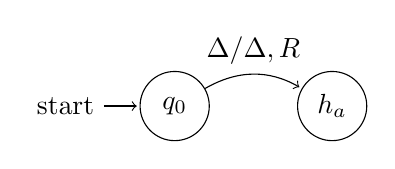
\begin{tikzpicture}[shorten >= 1, node distance = 2cm, on grid, auto]
    \node[state, initial] (0) {$q_0$};
    \node[state] (h) [right=of 0] {$h_a$};
    \path[->]
        (0) edge [bend left] node {$\Delta / \Delta , R$} (h);
    \end{tikzpicture}
    \caption{Transition diagram of a small Turing machine}
    \label{fig:TM2}
\end{wrapfigure}
If you want to have your figure beside your text you need to put it into a \emph{wrapfigure} instead of a normal \emph{figure}. Place the text at the line, on which you want the figure to start. The first variable are the amount of lines the box is high, the second is left or right, while the last is the width.

\section{Tables}
Tables are also put into a float similar to figures, which makes it possible to add captions and references to it similar to before, such as the table in \ref{tab:table}. The table itself is made with \emph{tabular}.
\begin{table}[h!]
    \centering
    \begin{tabular}{ l r | c || >{\columncolor[gray]{0.5}}c >{\columncolor[RGB]{230, 242, 255}}c}
        \rowcolor{lstKey2} %color defined for code highlights
        l-column           & r-column & c-column                  & gray column & light blue column
    \\ \hline \hline % horizontal lines
        a                  & b        & c                         & d           & e
    \\ \hline
        f                  & g        & \cellcolor[HTML]{FFCE93}h & i           & j
    \\
        $k = \frac{1}{2}$  & l        & m                         & n           & o
    \end{tabular}
    \caption{A table with this being the caption}
    \label{tab:table}
\end{table}

\newpage
\section{Graphs}
Here is a graph from our first Calculus handin, kindly sponsored by the wonderful Rasmus Skovdal. \cite{rasmus} This can also be inserted into a figure, with which there are also captions and reference options.

\begin{center}
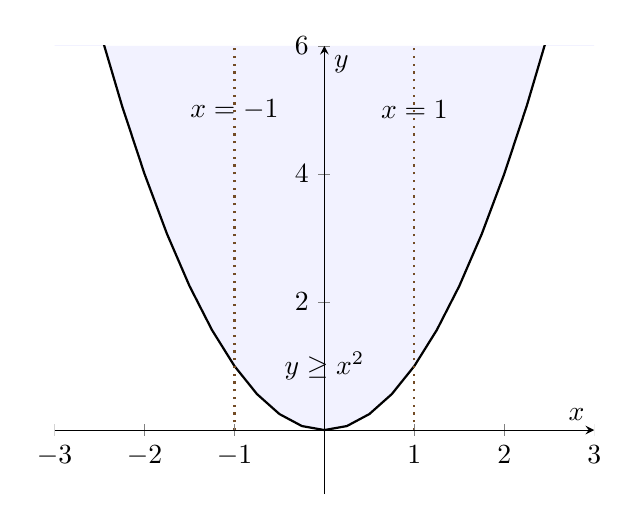
\begin{tikzpicture}
\begin{axis}[
    xmin=-3, xmax=3,
    ymin=-1, ymax=6,
    xlabel={$x$},ylabel={$y$},
    axis lines=center,
    axis on top=true,
    ]
    %Graf x^2
    \addplot [name path=f, domain=-3:3,black, thick] {x^2};
    %Øverste kant for fill
    \path[name path=axis] (axis cs:-3,6) -- (axis cs:3,6);
    %Indstillinger for fill
    \addplot [
        thick,
        color=blue,
        fill=blue, 
        fill opacity=0.05
    ]
    %Start af fill
    fill between[
        of=f and axis,
    ];
    
    %Tegner lodrette streger
    \addplot+[ycomb,dotted,thick,no marks] table[x=x,y expr=6] {
    x
    -1
    1
    };
    
    %Tilføjer tekst
    \node [] at (axis cs:  -1, 5) {$x=-1$};
    \node [] at (axis cs:  1, 5) {$x=1$};
    \node at (axis cs:  0, 1) {$y\geq x^2$};    
\end{axis}
\end{tikzpicture}
\end{center}

\section{Code}
The following is sourcecode for some non-aweinspiring Java method. By using a caption you also give it a number, but alternatively it can be given a \emph{title} instead of a \emph{caption}. Using \emph{title} does break the ability to make and reference a \emph{label}, but that is your intent anyways, if you use \emph{title}. The following code has the label \ref{lst:Example}

\begin{lstlisting} [language=java,
                    label={lst:Example},
                    caption={I'm a caption}]
//This is a comment, nordic letters are not supported
public static String example(int n) {
    return "You wrote: "+n;
}
\end{lstlisting}

If the language has to be something else than is the standard specified, then it has to be declared as an argument. In the following pseudocode there are also used escape characters *@ and @* to insert \LaTeX\ math.

\begin{lstlisting}[firstnumber=1,
                   caption={The algorithm \emph{linear exponentiation}},
                   label={lst:algorithm}]
*@ \textbf{Algorithm: Linear Exponentiation} @*(x,p)
 Input     : *@ $p \geq 0$ @*
 Output    : *@ $r = x^p$ @*
 Method    : *@ $r \leftarrow 1$ @*
             *@ $q \leftarrow p$ @*
              {I} while *@ $q > 0$ @* do
                    *@ $r \leftarrow r * x$ @*
                    *@ $q \leftarrow q - 1$ @*
\end{lstlisting}

\newpage
\section{Trees}
With qtree we have a quick and easy way to draw trees. Notice, that you need to have a space between an element and a closing bracket.
\begin{figure}[htbp]
    \centering
    \Tree [.rod [.{rod for et subtræ}
                blad
                blad ]
            blad ]
    \caption{A tree}
    \label{fig:tree1}
\end{figure}

If the trees need to be a bit more complex, then you need to use tikz, where it is already in the preamble has defined red-black trees.
\begin{figure}[htbp]
    \centering
    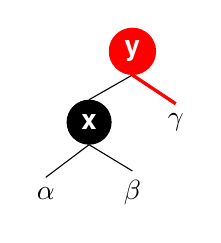
\begin{tikzpicture}[baseline={(current bounding box.center)},-,>=stealth',level/.style={sibling distance = 1.1cm, level distance = 0.9cm}]
            \node [arn_r] {y}
                child{ node [arn_b] {x} 
                    child{ node {$\alpha$} }
                    child{ node {$\beta$} }                            
                }
                child[style={edge from parent/.style={red,very thick,draw}}]
                    { node {$\gamma$} }
            ;
    \end{tikzpicture}
    \caption{A nicer tree}
    \label{fig:tree2}
\end{figure}

\section{Automata}
By using Tikz creating automota by hand is easy, and I highly encourage you do it manually, to make modifications later much easier and your document much nicer in general. In the following the only complication has been the longer edge from (C) to (A) over 1, where in the code commented out it is explicitly defined by guiding points, but it could also be done by changing the angle, which is by default 30 degrees.
\begin{figure}[htbp]
    \centering
    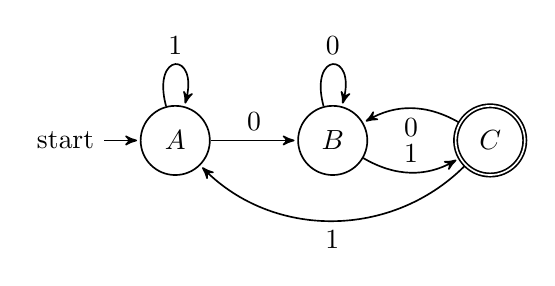
\begin{tikzpicture}[>=stealth', semithick,                                  % More pronounced edges
                        shorten >= 1, node distance = 2cm, on grid, auto]       % Node placement settings
    \node[state, initial] (A) {$A$};
    \node[state] (B) [right=of A] {$B$};
    \node[state, accepting] (C) [right=of B] {$C$};
    \path[->]
        (A) edge node {0} (B)
            edge [loop above] node {1} ()
        (B)    edge [loop above] node {0} ()
            edge [bend right] node {1} (C)
        (C)    edge [bend left=45] node {1} (A)
            edge [bend right] node {0} (B);
    %\draw[->] (C) .. controls ($(C)+(0,-1cm)$) and ($(A)+(0,-1cm)$).. (A)      % Custom edge
    %                node at ($(B)+(0,-1.1cm)$) {$1$};
    \end{tikzpicture}
    \caption{A finite automoata, that accepts strings ending with "01"}
    \label{fig:FA}
\end{figure}

\newpage
\section{E/R Diagrams} \label{sec:ER}
By using \emph{er} and \emph{shapes} packages a E/R diagram can be drawn. These are made in the exact same way as the automota.

\begin{figure}[htbp!]
    \centering
    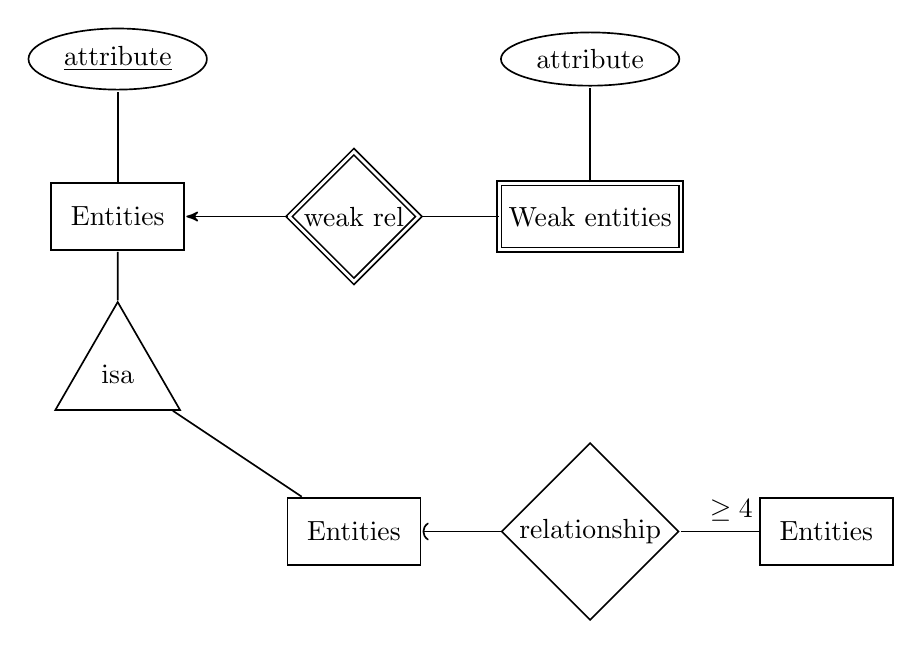
\begin{tikzpicture}[>=stealth', semithick,                                                  % More pronounced edges
                        shorten >= 0.5, node distance = 2cm and 3cm, on grid, auto,             % Node placement settings
                        isa/.style = {regular polygon, regular polygon sides=3, draw=black}]    % Defining isa nodes
        \node[entity] (ent1) {Entities};
        \node[attribute] (attr1) [above =of ent1] {\underline{attribute}};
        \node[relationship, double distance=0.1em] (wrel) [right =of ent1] {weak rel};
        \node[entity, double distance=0.1em] (went) [right =of wrel] {Weak entities};
        \node[attribute] (attr2) [above =of went] {attribute};
        \node[isa] (isa) [below =of ent1] {isa};
        \node[entity] (ent2) [below right =of isa] {Entities};
        \node[relationship] (rel1) [right =of ent2] {relationship};
        \node[entity] (ent3) [right =of rel1] {Entities};
        %edge:many
        \path[-]
            (ent1) edge (attr1)
            (went) edge (wrel)
            (went) edge (attr2)
            (isa) edge (ent1)
            (isa) edge (ent2)
            (ent3) edge node [above, pos = 0.35] {$\geq 4$} (rel1);
        %edge:one
        \path[->]
            (wrel) edge (ent1);
        %edge:exactly-one
        \path[-)]
            (rel1) edge (ent2);
    \end{tikzpicture}
    \label{fig:ER}
\end{figure}

\section{Referencing and Citing} \label{sec:ref}
If you need to reference equations, figures, sections or anything with a label you want to use the \emph{ref} operation. A \emph{ref} will always point to a \emph{label} defined and saved in the earlier compilation. For example this section has the number \ref{sec:ref}.

If you wan to reference the bibliography, then you want to use the \emph{cite} operation instead. Here is a reference to \cite{berlog}, which is written in the \emph{bibliography} further down. This is redefined to litteratur with the danish preamble, preamble\_dk.tex. If you want more references simultaneously you just seperate them with commas: \cite{berlog, steffan}

\section{Quotes}
With the \emph{csquotes} package it is possible to make nice quotes, such as Steffan's remark \textcquote[s. 12]{steffan}{We are computer scientists, not vampires}. By using \emph{blockquote} you get automatically a quote, which is on its own line, if it is 4+ lines long.

\blockcquote[s. 1]{berlog}{Lorem ipsum dolor sit amet, consectetur adipiscing elit, sed do eiusmod tempor incididunt ut labore et dolore magna aliqua. Ut enim ad minim veniam, quis nostrud exercitation ullamco laboris nisi ut aliquip ex ea commodo consequat. Duis aute irure dolor in reprehenderit in voluptate velit esse cillum dolore eu fugiat nulla pariatur.}

Notice, that both quotes used a \emph{c} as a prefix to \emph{quote}. This gives the possibility to reference to the bibliography. If you don't need that you can safely remove it.

\section{Columns}
\begin{multicols}{2}

\noindent Here is some text split into two columns, which can be used for various things. I have not used this very often, so I'm not sure if it works well with various stuff prior shown, such as figures, code or equations. If you want to use code, you will have to at least not include a header and remove the centering option as set up in the preamble.

\vfill \columnbreak

Here is some more text in the other column. Over here we could have the index, while on the other side we have the title and also the abstract?

\end{multicols}

\begin{thebibliography}{9}
\bibitem{rasmus}
    Skovdal, Rasmus: \emph{Calculus 1}, 2015
\bibitem{steffan}
    Jørgensen, Steffan: \emph{101 quotes}, 2015
\bibitem{berlog}
    Huth, Michael og Ryan, Mark: \emph{Logic in Computer Science}, second edition, 2004

\bibitem{referencer.bib}
 You can either write the bibliography in this document or have an extra references.bib file with all the information in the following form:
 
@book{FilVri97,
Author = {Filar, Jerzy and Vrieze, Koos},
Publisher = {Springer},
Title = {Competitive Markov Decision Processes},
Year = 1997
} 
 
\end{thebibliography}
\bibliographystyle{abbrv}
\bibliography{referencer}

\newpage
\appendix
\section{An Appendix}
Lorem ipsum dolor sit amet, consectetur adipiscing elit, sed do eiusmod tempor incididunt ut labore et dolore magna aliqua. Ut enim ad minim veniam, quis nostrud exercitation ullamco laboris nisi ut aliquip ex ea commodo consequat.

\end{document}
